\documentclass[12pt]{article}
\setlength{\textwidth}{17cm}
\setlength{\textheight}{24cm}
\setlength{\topmargin}{-2cm}
\setlength{\footskip}{1cm}
\setlength{\evensidemargin}{0cm}
\setlength{\oddsidemargin}{0cm}
\setlength{\parindent}{0cm}

\usepackage{allrunes}
\usepackage{amsmath}
\usepackage[magyar]{babel}
\usepackage[T1]{fontenc}
\usepackage[utf8]{inputenc}
\usepackage{fixltx2e}
\usepackage{multirow}

\usepackage[hyphens]{url}
\usepackage[unicode,colorlinks=true,breaklinks]{hyperref}
%\usepackage[dvips]{hyperref}
%should display links, but it does not work with \H accent
%and formulas in section titles

\hypersetup{colorlinks,linkcolor=blue,urlcolor=magenta,citecolor=magenta}
%Breaks long url`s in text, while keeping it one link:

\usepackage{amsfonts}
\usepackage{amsthm}
\usepackage{amssymb}


\theoremstyle{plain}
\usepackage{graphicx}

%\usepackage{gensymb}
\usepackage{float}

% For bra-ket notation
\usepackage{braket}

%% New commands
\newcommand{\dd}{\textrm{d}}

%% Pauli matrices
\newcommand{\sigx}{\sigma_x}
\newcommand{\sigy}{\sigma_y}
\newcommand{\sigz}{\sigma_z}

\newcommand{\paulix}{
    \left( \begin{array}{cc}
        0 & 1 \\
        1 & 0
    \end{array}
    \right)
}

\newcommand{\pauliy}{
    \left( \begin{array}{cc}
        0 & -i \\
        i & 0
    \end{array}
    \right)
}

\newcommand{\pauliz}{
    \left( \begin{array}{cc}
        1 & 0 \\
        0 & -1
    \end{array}
    \right)
}


\begin{document}
\title{13. tétel}
\author{Kruppa Zoltán}

\maketitle

\pagenumbering{gobble}

\begin{abstract}
    \centering
    Dimenzióredukciós módszerek – Magas dimenziós adatok statisztikus tulajdonságai. A főkomponens-analízis és alkalmazásai, t-SNE.
\end{abstract}

\vfill

\tableofcontents

\newpage

\section{Introduction}

In statistics, machine learning, and information theory, dimensionality reduction or dimension reduction is the process of reducing the number of random variables under consideration by obtaining a set of principal variables. It can be divided into feature selection and feature extraction.\cite{wiki_dim}

\section{Dimension Reduction\cite{dim_red}}
\subsection{What are Dimension Reduction techniques?}

Dimension Reduction refers to the process of converting a set of data having vast dimensions into data with lesser dimensions ensuring that it conveys similar information concisely. These techniques are typically used while solving \textbf{machine learning problems} to obtain better features for a classification or regression task.
\\

Let’s look at the image shown below (Fig~\ref{fig:ss}). It shows $2$ dimensions $x_1$ and $x_2$, which are let us say measurements of several object in cm ($x_1$) and inches ($x_2$). Now, if you were to use both these dimensions in machine learning, they will convey similar information and introduce a lot of noise in system, so you are better of just using one dimension. Here we have converted the dimension of data from $2D$ $($from $x_1$ and $x_2)$ to $1D$ $(z_1)$, which has made the data relatively easier to explain.
\\

\begin{figure}[h!]
 \begin{center}
  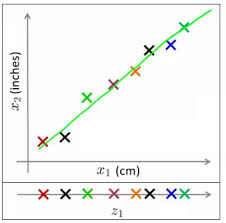
\includegraphics[width=0.3\textwidth]{media/2D_1D.png}
  \caption{Measurements of several object in cm}  
\label{fig:ss}
 \end{center}

\end{figure}

In similar ways, we can reduce $n$ dimensions of data set to k dimensions $(k < n)$ . These k dimensions can be directly identified (filtered) or can be a combination of dimensions (weighted averages of dimensions) or new dimension(s) that represent existing multiple dimensions well.
\\

One of the most common application of this technique is \textbf{Image processing}. You might have come across this Facebook application – \underline{"Which Celebrity Do You Look Like?"}. But, have you ever thought about the algorithm used behind this?

\underline{Here's the answer:} To identify the matched celebrity image, we use pixel data and each pixel is equivalent to one dimension. In every image, there are high number of pixels i.e. high number of dimensions. And every dimension is important here. You can’t omit dimensions randomly to make better sense of your overall data set. In such cases, dimension reduction techniques help you to find the significant dimension(s) using various method(s). We’ll discuss these methods shortly.

\subsection{What are the benefits of Dimension Reduction?}

Let’s look at the benefits of applying Dimension Reduction process:

\begin{itemize}
\item It helps in data compressing and reducing the storage space required
\item It fastens the time required for performing same computations. Less dimensions leads to less computing, also less dimensions can allow usage of algorithms unfit for a large number of dimensions
\item It takes care of multi-collinearity that improves the model performance. It removes redundant features. For example: there is no point in storing a value in two different units (meters and inches).
\item Reducing the dimensions of data to $2D$ or $3D$ may allow us to plot and visualize it precisely. You can then observe patterns more clearly. Below you can see that, how a $3D$ data is converted into $2D$. First it has identified the $2D$ plane then represented the points on these two new axis $z_1$ and $z_2$.
\end{itemize}

\begin{figure}[H]
 \begin{center}
  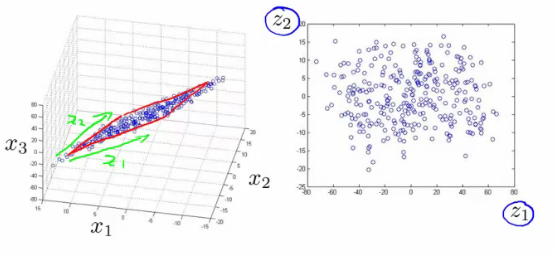
\includegraphics[width=0.6\textwidth]{media/Image-4.png}

 \end{center}
\end{figure}

\begin{itemize}
\item It is helpful in noise removal also and as result of that we can improve the performance of models.
\end{itemize}

\subsection{What are the common methods to perform Dimension Reduction?}

There are many methods to perform Dimension reduction. I have listed the most common methods below:

\begin{enumerate}
\item  \textbf{Missing Values:} While exploring data, if we encounter missing values, what we do? Our first step should be to identify the reason then impute missing values/ drop variables using appropriate methods. But, what if we have too many missing values? Should we impute missing values or drop the variables?
\item  \textbf{Low Variance:} Let’s think of a scenario where we have a constant variable (all observations have same value, 5) in our data set. Do you think, it can improve the power of model? Of course NOT, because it has zero variance. In case of high number of dimensions, we should drop variables having low variance compared to others because these variables will not explain the variation in target variables.
\item  \textbf{Decision Trees:} It can be used as a ultimate solution to tackle multiple challenges like missing values, outliers and identifying significant variables. It worked well in our Data Hackathon also. Several data scientists used decision tree and it worked well for them.
\item  \textbf{Random Forest:} Similar to decision tree is Random Forest. It would also be recommend using the in-built feature importance provided by random forests to select a smaller subset of input features. Just be careful that random forests have a tendency to bias towards variables that have more no. of distinct values i.e. favor numeric variables over binary/categorical values.
\item  \textbf{Factor Analysis:} Let’s say some variables are highly correlated. These variables can be grouped by their correlations i.e. all variables in a particular group can be highly correlated among themselves but have low correlation with variables of other group(s). Here each group represents a single underlying construct or factor. These factors are small in number as compared to large number of dimensions. However, these factors are difficult to observe. There are basically two methods of performing factor analysis:
	\begin{itemize}
	\item EFA (Exploratory Factor Analysis)
	\item CFA (Confirmatory Factor Analysis)
 	\end{itemize}
\item  \textbf{Principal Component Analysis (PCA):} In this technique, variables are transformed into a new set of variables, which are linear combination of original variables. These new set of variables are known as \textbf{principle components}. They are obtained in such a way that first principle component accounts for most of the possible variation of original data after which each succeeding component has the highest possible variance.

The second principal component must be orthogonal to the first principal component. In other words, it does its best to capture the variance in the data that is not captured by the first principal component. For two-dimensional dataset, there can be only two principal components. Below is a snapshot of the data and its first and second principal components. You can notice that second principle component is orthogonal to first principle component.

\begin{figure}[H]
 \begin{center}
  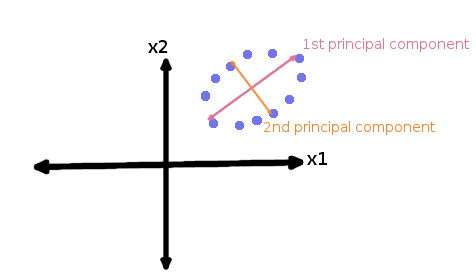
\includegraphics[width=0.6\textwidth]{media/PCA.png}

 \end{center}
\end{figure}

The principal components are sensitive to the scale of measurement, now to fix this issue we should always standardize variables before applying PCA. Applying PCA to your data set loses its meaning. If interpretability of the results is important for your analysis, PCA is not the right technique for your project.

\end{enumerate}

\section{Principal component analysis}
I wrote this chapter based on the Mark Richardson's note\cite{pca}.

Assume that we start with a data set that is represented in terms of an $m \times n$ matrix, $\textbf{X}$ where the $n$ columns are the samples (e.g. observations) and the $m$ rows are the variables. We wish to linearly transform this matrix,  $\textbf{X}$ into another matrix,  $\textbf{Y}$, also of dimension $m \times n$, so that for some $m \times m$ matrix, $\textbf{P}$,

\begin{equation}
\textbf{Y}=\textbf{PX}
\end{equation}

This equation represents a change of basis. If we consider the \emph{rows} of $\textbf{P}$ to be the row vectors $\textbf{p}_1 \textbf{p}_2, \cdots \textbf{p}_m$, and the \emph{columns} of \textbf{X} to be the column vectors $\textbf{x}_1, \textbf{x}_2,\cdots ,\textbf{x}_n$, then can be interpreted in the following way.

\begin{equation}
\textbf{PX} = (\textbf{Px}_1, \textbf{Px}_2 \cdots \textbf{Px}_n) = 
 \begin{pmatrix}
 \textbf{p}_1\textbf{x}_1  & \textbf{p}_1\textbf{x}_2 & \cdots & \textbf{p}_1\textbf{x}_n \\
 \textbf{p}_2\textbf{x}_1  & \textbf{p}_2\textbf{x}_2 & \cdots & \textbf{p}_2\textbf{x}_n \\
  \vdots  & \vdots  & \ddots & \vdots  \\
\textbf{p}_m\textbf{x}_1  & \textbf{p}_m\textbf{x}_2 & \cdots & \textbf{p}_m\textbf{x}_n
 \end{pmatrix}
= \textbf{Y}
\end{equation}


Note that $p_i , x_j \in \mathbb{R}^m$, and so $\textbf{p}_i\textbf{x}_j$ is just the standard Euclidean inner (dot) product. This tells us that the original data, \textbf{X} is being projected on to the \emph{columns} of \textbf{P}. Thus, the rows of \textbf{P}, $\{\textbf{p}_1 \textbf{p}_2, \cdots \textbf{p}_m\}$ are a new basis for representing the columns of X. The rows of \textbf{P} will later become our principal component directions
\\

We now need to address the issue of what this new basis should be, indeed what is the 'best' way to re-express the data in \textbf{X} - in other words, how should we define \emph{independence} between principal components in the new basis?
\\

Principal component analysis defines independence by considering the variance of the data
in the original basis. It seeks to de-correlate the original data by finding the directions in
which variance is maximised and then use these directions to define the new basis. Recall
the definition for the variance of a random variable, \emph{Z} with mean, $\mu$.

\begin{equation}
\sigma_Z^2 = E((Z-\mu)^2)
\end{equation}

Suppose we have a vector of $n$ discrete measurements, $\widetilde{\textbf{r}} = (\widetilde{r}_1, \widetilde{r}_2,\cdots, \widetilde{r}_n)$, with mean $\mu_r$. If we subtract the mean from each of the measurements, then we obtain a translated set of measurements $\textbf{r} = (r_1, r_2, \cdots , r_n)$, that has zero mean. Thus, the variance of these measurements is given by the relation
\begin{equation}
\sigma_r^2 = \frac{1}{n}\textbf{rr}^T
\end{equation}

If we have a second vector of $n$ measurements, $\textbf{s} = (s_1, s_2, \cdots , s_n)$, again with zero mean, then we can generalise this idea to obtain the \emph{covariance} of \textbf{r} and \textbf{s}. Covariance can be thought of as a measure of how much two variables change together. Variance is thus a special case of covariance, when the the two variables are identical. It is in fact correct to divide through by a factor of $n-1$ rather than $n$, a fact which we shall not justify here.

\begin{equation}
\sigma_{rs}^2=\frac{1}{n-1}\textbf{rs}^T
\end{equation}

We can now generalise this idea to considering our $m \times n$ data matrix, \textbf{X}. Recall that $m$ was the number of variables, and $n$ the number of samples. We can therefore think of this matrix, \textbf{X} in terms of $m$ row vectors, each of length $n$.

\begin{equation}
\textbf{X} = 
 \begin{pmatrix}
  x_{1,1} &x_{1,2} & \cdots & x_{1,n} \\
  x_{2,1} & x_{2,2} & \cdots &x_{2,n} \\
  \vdots  & \vdots  & \ddots & \vdots  \\
  x_{m,1} & a_{m,2} & \cdots & x_{m,n} 
 \end{pmatrix} =
\begin{pmatrix}
   \textbf{x}_1 \\
  \textbf{x}_2 \\
  \vdots   \\
 \textbf{x}_m 
 \end{pmatrix} \in \mathbb{R}^{m\times n}, \textbf{x}_1^T \in \mathbb{R}^n
\end{equation}

Since we have a row vector for each variable, each of these vectors contains all the samples
for one particular variable. So for example,  $\textbf{x}_i$ is a vector of the $n$ samples for the $i^th$ variable. It therefore makes sense to consider the following matrix product.

\begin{equation}
\textbf{C}_{\textbf{X}}= \frac{1}{1-n}\textbf{XX}^T=\frac{1}{1-n}
 \begin{pmatrix}
 \textbf{x}_1\textbf{x}_1^T  & \textbf{x}_1\textbf{x}_2^T & \cdots & \textbf{x}_1\textbf{x}_n^T \\
 \textbf{x}_2\textbf{x}_1^T  & \textbf{x}_2\textbf{x}_2^T & \cdots & \textbf{x}_2\textbf{x}_n^T \\
  \vdots  & \vdots  & \ddots & \vdots  \\
\textbf{x}_m\textbf{x}_1^T  & \textbf{x}_m\textbf{x}_2^T & \cdots & \textbf{x}_m\textbf{x}_n^T
 \end{pmatrix} \in \mathbb{R}^{m\times n}
\end{equation}

If we look closely at the entries of this matrix, we see that we have computed all the possible covariance pairs between the $m$ variables. Indeed, on the diagonal entries, we have the variances and on the off-diagonal entries, we have the \emph{covariances}. This matrix is therefore known as the \emph{Covariance Matrix.}
\\

Now let us return to the original problem, that of linearly transforming the original data matrix using the relation \textbf{Y}=\textbf{PX}, for some matrix, \textbf{P}. We need to decide upon some features that we would like the transformed matrix, \textbf{Y} to exhibit and somehow relate this to the features of the corresponding covariance matrix $\textbf{C}_{\textbf{Y}}$.
\\

Covariance can be considered to be a measure of how well correlated two variables are. The PCA method makes the fundamental assumption that the variables in the transformed matrix should be as uncorrelated as possible. This is equivalent to saying that the covariances of different variables in the matrix $\textbf{C}_{\textbf{Y}}$, should be as close to zero as possible (covariance matrices are always positive definite or positive semi-definite). Conversely, large variance values interest us, since they correspond to interesting dynamics in the system (small variances may well be noise). We therefore have the following requirements for constructing the covariance matrix, $\textbf{C}_{\textbf{Y}}$:
\begin{enumerate}
\item  Maximise the signal, measured by variance (maximise the diagonal entries)
\item  Minimise the covariance between variables (minimise the off-diagonal entries)
\end{enumerate}

We thus come to the conclusion that since the minimum possible covariance is zero, we are seeking a diagonal matrix, $\textbf{C}_{\textbf{Y}}$. If we can choose the transformation matrix, \textbf{P} in such a way that $\textbf{C}_{\textbf{Y}}$ is diagonal, then we will have achieved our objective.
\\

We now make the assumption that the vectors in the new basis, $\textbf{p}_1 \textbf{p}_2, \cdots \textbf{p}_m$ are orthogonal (in fact, we additionally assume that they are orthonormal). Far from being restrictive, this assumption enables us to proceed by using the tools of linear algebra to find a solution to the problem. Consider the formula for the covariance matrix, $\textbf{C}_{\textbf{Y}}$ and our interpretation of \textbf{Y} in terms of \textbf{X} and \textbf{P}.

\begin{equation}
\begin{split}
\textbf{C}_{\textbf{Y}}= \frac{1}{1-n}\textbf{XX}^T=\frac{1}{1-n}(\textbf{PX})(\textbf{PX})^T =\frac{1}{1-n}(\textbf{PX})(\textbf{P}^T\textbf{X}^T)
=\frac{1}{1-n}\textbf{P}(\textbf{XX}^T)\textbf{P}^T \\
 i.e. \hspace{0.5cm}\textbf{C}_{\textbf{Y}} =  \frac{1}{1-n}\textbf{PSP}^T \hspace{0.5cm} where \hspace{0.5cm} S=\textbf{XX}^T
\end{split}
\end{equation}

Note that \textbf{S} is an $m\times m$ symmetric matrix, since $(\textbf{XX}^T)^T = (\textbf{X}^T)^T(\textbf{XX}^T)=\textbf{XX}^T$ . We now invoke the well known theorem from linear algebra that every square symmetric matrix is orthogonally (orthonormally) diagonalisable. That is, we can write:

\begin{equation}
\textbf{S}= \textbf{EDE}^T
\end{equation}

Where\textbf{E} is an $m\times m$ orthonormal matrix whose columns are the orthonormal eigenvectors of \textbf{S}, and \textbf{D} is a diagonal matrix which has the eigenvalues of \textbf{S} as its (diagonal) entries. The rank, $ r$, of \textbf{S} is the number of orthonormal eigenvectors that it has. If B turns out to be rank-deficient so that r is less than the size, m, of the matrix, then we simply need to generate $m-r$ orthonormal vectors to fill the remaining columns of \textbf{S}.
\\

It is at this point that we make a choice for the transformation matrix, \textbf{P}. By choosing
the \emph{rows} of \textbf{P} to be the eigenvectors of \textbf{S}, we ensure that $\textbf{P}= \textbf{E}^T$ and vice-versa. Thus, substituting this into our derived expression for the covariance matrix, $\textbf{C}_{\textbf{Y}}$ gives:

\begin{equation}
\textbf{C}_{\textbf{Y}} =  \frac{1}{1-n}\textbf{PSP}^T =\frac{1}{1-n}\textbf{E}^T(\textbf{EDE}^T)\textbf{E}
\end{equation}

Now, since \textbf{E} is an orthonormal matrix, we have $\textbf{E}^T\textbf{E} = \textbf{I}$, where  \textbf{I} is the $m \times m$ identity matrix. Hence, for this special choice of  \textbf{P}, we have:

\begin{equation}
\textbf{C}_{\textbf{Y}} =  \frac{1}{1-n}\textbf{D}
\end{equation}


A last point to note is that with this method, we automatically gain information about the relative importance of each principal component from the variances. The largest variance corresponds to the first principal component, the second largest to the second principal component, and so on. This therefore gives us a method for organising the data in the diagonalisation stage. Once we have obtained the eigenvalues and eigenvectors of  $\textbf{S} = \textbf{XX}^T$ , we sort the eigenvalues in descending order and place them in this order on the diagonal of \textbf{D}. We then construct the orthonormal matrix,\textbf{E} by placing the associated eigenvectors in the same order to form the columns of \textbf{E} (i.e. place the eigenvector that corresponds to the largest eigenvalue in the first column, the eigenvector corresponding to the second largest eigenvalue in the second column etc.).
\\

We have therefore achieved our objective of diagonalising the covariance matrix of the transformed data. The principal components (the rows of \textbf{P}) are the eigenvectors of the covariance matrix, $\textbf{XX}^T$ , and the rows are in order of 'importance', telling us how 'principal' each principal component is.

\subsection{The Singular Value Decomposition}

In this section, we will examine how the well known singular value decomposition (SVD) from linear algebra can be used in principal component analysis. Indeed, we will show that the derivation of PCA in the previous section and the SVD are closely related. We will not derive the SVD, as it is a well established result, and can be found in any good book on numerical linear algebra.
\\

Given $\textbf{A} \in \mathbb{R}^{n\times m}$, not necessarily of full rank, a singular value decomposition of \textbf{A} is:

\begin{equation}
\textbf{A} =\textbf{U}\mathbf{\Sigma}\textbf{V}^T
\end{equation}

Where
$$ \textbf{U} \in \mathbb{R}^{n\times n}  \hspace{0.5cm} is \hspace{0.3cm}orthonormal $$
$$ \mathbf{\Sigma} \in \mathbb{R}^{n\times m}  \hspace{0.5cm} is \hspace{0.3cm} diagonal $$
$$ \textbf{V} \in \mathbb{R}^{m\times m}  \hspace{0.5cm} is \hspace{0.3cm} orthonormal $$

In addition, the diagonal entries, $\sigma_i$, of $\Sigma$ are non-negative and are called the \emph{singular} values of \textbf{A}. They are ordered such that the largest singular value, $\sigma_1$ is placed in the (1, 1) entry of $\Sigma$, and the other singular values are placed in order down the diagonal, and satisfy $\sigma_1 \geq \sigma_2 \geq  \cdots \sigma_p \geq 0$, where $p = min(n, m)$. Note that we have reversed the row and column indexes in defining the SVD from the way they were defined in the derivation of PCA in the previous section. The reason for doing this will become apparent shortly.
\\


Since $\textbf{U} \in \mathbb{R}^{n\times n}$ and $\textbf{V} \in \mathbb{R}^{m\times m}$ are orthonormal matrices, their columns form bases for, respectively, the vector spaces $\mathbb{R}^n$ and $\mathbb{R}^m$. Therefore, any vector $\textbf{b} \in \mathbb{R}^n$ can be expanded in the basis formed by the columns of \textbf{U} (also known as the \emph{left singular vectors} of \textbf{A}) and any vector $\textbf{x} \in \mathbb{R}^m$ can be expanded in the basis formed by the columns of \textbf{V} (also known as the \emph{right singular vectors} of \textbf{A}). The vectors for these expansions $\hat{\textbf{b}}$ and $\hat{\textbf{x}}$, are given by:

\begin{equation}
\hat{\textbf{b}} = \textbf{U}^T\textbf{b}  \hspace{0.5cm} and  \hspace{0.5cm} \hat{\textbf{x}} = \textbf{V}^T\textbf{x}
\end{equation}

Now, if the relation \textbf{b} = \textbf{Ax} holds, then we can infer the following:

\begin{equation}
\textbf{U}^T\textbf{b} = \textbf{U}^T\textbf{Ax} \rightarrow \hat{\textbf{b}} = \textbf{U}^T(\textbf{U}\mathbf{\Sigma}\textbf{V}^T)\textbf{x}  \rightarrow \hat{\textbf{b}} = \mathbf{\Sigma}\hat{\textbf{x}}
\end{equation}

Thus, the SVD allows us to assert that every matrix is diagonal, so long as we choose the appropriate bases for the domain and range spaces.
\\

How does this link in to the previous analysis of PCA? Consider the $n\times m$ matrix, \textbf{A}, for which we have a singular value decomposition,$\textbf{A} =\textbf{U}\mathbf{\Sigma}\textbf{V}^T$. There is a theorem from linear algebra which says that the non-zero singular values of \textbf{A} are the square roots of the
nonzero eigenvalues of $\textbf{A}\textbf{A}^T$ or $\textbf{A}^T\textbf{A}$. The former assertion for the case $\textbf{A}^T\textbf{A}$ is proven in the following way:

\begin{equation}
\textbf{A}^T\textbf{A}=(\textbf{U}\mathbf{\Sigma}\textbf{V}^T)^T(\textbf{U}\mathbf{\Sigma}\textbf{V}^T)=
(\textbf{U}\mathbf{\Sigma}^T\textbf{V}^T)(\textbf{U}\mathbf{\Sigma}\textbf{V}^T)=
\textbf{V}(\mathbf{\Sigma}^T\mathbf{\Sigma})\textbf{V}^T
\end{equation}

We observe that $\textbf{A}^T\textbf{A}$ is similar to $\mathbf{\Sigma}^T\mathbf{\Sigma}$, and thus it has the same eigenvalues. Since $\mathbf{\Sigma}^T\mathbf{\Sigma}$ is a square $(m\times m)$, diagonal matrix, the eigenvalues are in fact the diagonal entries, which are the squares of the singular values. Note that the nonzero eigenvalues of each of the covariance matrices, $\textbf{A}\textbf{A}^T$ and $\textbf{A}^T\textbf{A}$ are actually identical.
\\


It should also be noted that we have effectively performed an eigenvalue decomposition for the matrix,  $\textbf{A}^T\textbf{A}$. Indeed, since  $\textbf{A}^T\textbf{A}$ is symmetric, this is an orthogonal diagonalisation
and thus the eigenvectors of  $\textbf{A}^T\textbf{A}$ are the columns of \textbf{V}. This will be important in making
the practical connection between the SVD and and the PCA of matrix \textbf{X}, which is what we will do next.
\\

Returning to the original $m\times n$ data matrix, \textbf{X}, let us define a new $n\times m$ matrix, \textbf{Z}:

\begin{equation}
\textbf{Z} = \frac{1}{\sqrt{1-n}}\textbf{X}^T
\end{equation}

Recall that since the m rows of \textbf{X} contained the n data samples, we subtracted the row average from each entry to ensure zero mean across the rows. Thus, the new matrix, \textbf{Z} has \emph{columns} with zero mean. Consider forming the $m\times m$ matrix, $\textbf{Z}^T\textbf{Z}$:

\begin{equation}
\begin{split}
\textbf{Z}^T\textbf{Z} = (\frac{1}{\sqrt{1-n}}\textbf{X}^T)^T(\frac{1}{\sqrt{1-n}}\textbf{X}^T)= \frac{1}{{1-n}}\textbf{X}\textbf{X}^T \\
i.e.  \hspace{0.9cm} \textbf{Z}^T\textbf{Z} = \textbf{C}_{\textbf{X}}
\end{split}
\end{equation}

We find that defining \textbf{Z} in this way ensures that $\textbf{Z}^T\textbf{Z}$ is equal to the covariance matrix of \textbf{X}, $\textbf{C}_{\textbf{X}}$. From the discussion in the previous section, the principal components of \textbf{X} (which is what we are trying to identify) are the eigenvectors of  $\textbf{C}_{\textbf{X}}$. Therefore, if we perform a singular value decomposition of the matrix $\textbf{Z}^T\textbf{Z}$, the principal components will be the columns of the orthogonal matrix, \textbf{V}.
\\


The last step is to relate the SVD of $\textbf{Z}^T\textbf{Z}$ back to the change of basis represented by equation:


\begin{equation}
\textbf{Y}=\textbf{PX}
\end{equation}

We wish to \emph{project} the original data onto the directions described by the principal components. Since we have the relation $\textbf{V}=\textbf{P}^T$, this is simply:

\begin{equation}
\textbf{Y}=\textbf{V}^T\textbf{X}
\end{equation}

If we wish to recover the original data, we simply compute (using orthogonality of \textbf{V}):

\begin{equation}
\textbf{X}=\textbf{V}^T\textbf{Y}
\end{equation}

\subsection{Applications}

\subsubsection{Quantitative finance}
In quantitative finance, principal component analysis can be directly applied to the risk management of interest rate derivative portfolios. Trading multiple swap instruments which are usually a function of 30-500 other market quotable swap instruments is sought to be reduced to usually 3 or 4 principal components, representing the path of interest rates on a macro basis. Converting risks to be represented as those to factor loadings (or multipliers) provides assessments and understanding beyond that available to simply collectively viewing risks to individual 30-500 buckets.
\\


PCA has also been applied to share portfolios in a similar fashion, both to portfolio risk and to risk return. One application is to reduce portfolio risk, where allocation strategies are applied to the "principal portfolios" instead of the underlying stocks. A second is to enhance portfolio return, using the principal components to select stocks with upside potential

\subsubsection{Neuroscience}

A variant of principal components analysis is used in neuroscience to identify the specific properties of a stimulus that increase a neuron's probability of generating an action potential. This technique is known as spike-triggered covariance analysis. In a typical application an experimenter presents a white noise process as a stimulus (usually either as a sensory input to a test subject, or as a current injected directly into the neuron) and records a train of action potentials, or spikes, produced by the neuron as a result. Presumably, certain features of the stimulus make the neuron more likely to spike. In order to extract these features, the experimenter calculates the covariance matrix of the spike-triggered ensemble, the set of all stimuli (defined and discretized over a finite time window, typically on the order of 100 ms) that immediately preceded a spike. The eigenvectors of the difference between the spike-triggered covariance matrix and the covariance matrix of the prior stimulus ensemble (the set of all stimuli, defined over the same length time window) then indicate the directions in the space of stimuli along which the variance of the spike-triggered ensemble differed the most from that of the prior stimulus ensemble. Specifically, the eigenvectors with the largest positive eigenvalues correspond to the directions along which the variance of the spike-triggered ensemble showed the largest positive change compared to the variance of the prior. Since these were the directions in which varying the stimulus led to a spike, they are often good approximations of the sought after relevant stimulus features.\cite{wiki_pca}
\\
 

In neuroscience, PCA is also used to discern the identity of a neuron from the shape of its action potential. Spike sorting is an important procedure because extracellular recording techniques often pick up signals from more than one neuron. In spike sorting, one first uses PCA to reduce the dimensionality of the space of action potential waveforms, and then performs clustering analysis to associate specific action potentials with individual neurons.
\\


PCA as a dimension reduction technique is particularly suited to detect coordinated activities of large neuronal ensembles. It has been used in determining collective variables, i.e. order parameters, during phase transitions in the brain.\cite{wiki_pca}

\section{t-distributed stochastic neighbor embedding}

This chapter summarizes the work of L. van der Maaten, and G. Hinton\cite{sne}.
\subsection{Stochastic Neighbor Embedding}

Stochastic Neighbor Embedding (SNE) starts by converting the high-dimensional Euclidean distances between datapoints into conditional probabilities that represent similarities. The similarity of datapoint $x_j$ to datapoint $x_j$ is the conditional probability, $p_{j|i}$, that $x_i$ would pick $x_j$ as its neighbor if neighbors were picked in proportion to their probability density under a Gaussian centered at $x_i$. For nearby datapoints, $p_{j|i}$ is relatively high, whereas for widely separated datapoints, $p_{j|i}$ will be almost infinitesimal. Mathematically, the conditional probability $p_{j|i}$ is given by

\begin{equation}
p_{j|i} = \frac{exp(-||x_i-x_j||^2/2\sigma_i^2)}{\sum_{k \neq i}exp(-||x_i-x_j||^2/2\sigma_i^2)}
\end{equation}


where $\sigma_i$ is the variance of the Gaussian that is centered on datapoint $x_i$. We set the value of $p_{i|i}$ to zero. For the low-dimensional counterparts $y_i$ and $y_j$ of the high-dimensional datapoints $x_i$ and $x_j$ , it is possible to compute a similar conditional probability, which we denote by $q_{j|i}$. We set the variance of the Gaussian that is employed in the computation of the conditional probabilities $q_{j|i}$. to $\frac{1}{\sqrt{2}}$. Hence, we model the similarity of map point $y_j$ to map point $y_i$ by

\begin{equation}
q_{j|i} = \frac{exp(-||x_i-x_j||^2)}{\sum_{k \neq i}exp(-||x_i-x_j||^2)}
\end{equation}

We set $q_{j|i} = 0$
\\


If the map points $y_i$ and $y_j$ correctly model the similarity between the high-dimensional datapoints $x_i$ and $x_j$ , the conditional probabilities $p_{j|i}$ and $q_{j|i}$ will be equal.
SNE finds a low-dimensional data representation by minimizing the inconsistency between $p_{j|i}$ and $q_{j|i}$. Furthermore, the Kullback–Leibler divergence method is used to measure the degree of accuracy in the way $q_{j|i}$ models $p_{j|i}$. SNE uses a gradient descent method to minimize the sum of Kullback–Leibler divergences over all data points that incurs some cost. The cost function $C$ is given by

\begin{equation}
C = \sum_i KL(P_i||Q_i)  = \sum_i\sum_j p_{j|i}log\frac{p_{j|i}}{q_{j|i}}
\end{equation}

in which $P_i$ represents the conditional probability distribution over all other datapoints given datapoint $x_i$, and $Q_i$ represents the conditional probability distribution over all other map points given map point $y_i$
\\

The remaining parameter to be selected is the variance $\sigma_i$ of the Gaussian that is centered over each high-dimensional datapoint, $x_i$. It is not likely that there is a single value of $\sigma_i$ that is optimal for all datapoints in the data set because the density of the data is likely to vary. In dense regions, a smaller value of $\sigma_i$ is usually more appropriate than in sparser regions. Any particular value of $\sigma_i$ induces a probability distribution, $P_i$, over all of the other datapoints. This distribution has an entropy which increases as $\sigma_i$ increases. SNE performs a binary search for the value of $\sigma_i$ that produces a $P_i$ with a fixed perplexity that is specified by the user. The perplexity is defined as

\begin{equation}
Prep(P_i)=2^{H(P_i)},
\end{equation}

where $H(P_i)$ is the Shannon entropy of Pi measured in bits

\begin{equation}
{H(P_i)}=-\sum_i p_{j|i}log_2 p_{j|i}
\end{equation}

\subsection{t-SNE}

In t-SNE, we employ a Student t-distribution with one degree of freedom (which is the same as a Cauchy distribution) as the heavy-tailed distribution in the low-dimensional map. Using this
distribution, the joint probabilities $q_{ij}$ are defined as

\begin{equation}
q_{ij}= \frac{(1+||x_i-x_j||^2)^{-1}}{\sum_{k \neq i}(1+||x_i-x_j||^2)^{-1}}
\label{qij}
\end{equation}


We use a Student t-distribution with a single degree of freedom, because it has the particularly nice property that $(1+||x_i-x_j||^2)^{-1}$ approaches an inverse square law for large pairwise distances. $||x_i-x_j||$ in the low-dimensional map.
\\


The gradient of the Kullback-Leibler divergence between P and the Student-t based joint probability distribution Q(Equation~\ref{qij}) is given by
\begin{equation}
\frac{\delta C}{\delta y_i} = 4\sum_j(p_{ij}-q_{ij})(y_i-y_j)(1+||x_i-x_j||^2)^{-1}
\end{equation}

\begin{figure}[h!]
 \begin{center}
  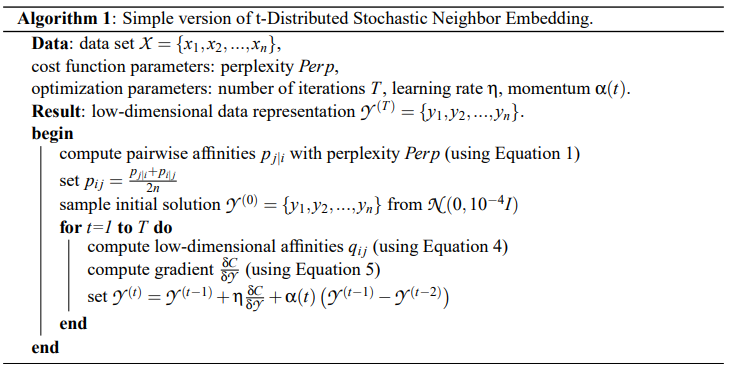
\includegraphics[width=0.9\textwidth]{media/alg.png}
 \end{center}
\end{figure}

\newpage

\vfill

\bibliographystyle{plain}
\bibliography{references}

\end{document}
